\exercice*

Considerar el trinomio de segundo grado $f: x\mapsto (( a|facteur("X") )) (( b|facteur("*sox") )) (( c|facteur("so") ))$.

\begin{enumerate}
\item
\begin{enumerate}
    \item Si $x\in\mathbb{R}$. Entonces :
        \begin{align*}
            (( a|facteur )) \,\left( x (( -x1|facteur("so") )) \right) \, \left( x (( -x2|facteur("so") )) \right)
            &= (( a|facteur )) \,\left(x\times{} x (( -x1|facteur("so") ))\times{} x (( -x2|facteur("so") ))\times{} x (( -x1|facteur("so") ))\times{} (( -x2|facteur("p") )) \right) \\
            &= (( a|facteur )) \,\left(x^2 (( (-x1-x2)|facteur("so*x") )) (( (x1*x2)|facteur("so*") ))\right) \\
            &= (( a|facteur ))\times{} x^2 (( a|facteur("so") ))\times{} (( (-x1-x2)|facteur("p*x") )) (( a|facteur("so") ))\times{} (( (x1*x2)|facteur("p") )) \\
            &= (( a|facteur("X") )) (( b|facteur("so*x") )) (( c|facteur("so") ))\\
            &= f\,(x)
        \end{align*}
    \item Si $x\in\mathbb{R}$. Entonces :
        \begin{align*}
            (( a|facteur ))\,\left( x (( -alpha|facteur("so") )) \right)^2 (( beta|facteur("so") ))
            &= (( a|facteur ))\,\left( x^2 (( (-signealpha*2)|facteur("so") ))\times{} (( absalpha|facteur )) \times{} x + (( absalpha|facteur ))^2\right) (( beta|facteur("so") ))\\
            &= (( a|facteur ))\,\left( x^2 (( (-alpha*2)|facteur("so*x") )) + (( (absalpha**2)|facteur ))\right) (( beta|facteur("so") ))\\
            &=  (( a|facteur ))\times{} x^2 (( a|facteur("so") ))\times{} (( (-alpha*2)|facteur("p*x") )) (( a|facteur("so") ))\times{} (( (absalpha**2)|facteur )) (( beta|facteur("so") ))\\
            &= (( a|facteur("X") )) (( b|facteur("so*x") )) (( (a*absalpha**2)|facteur("so") )) (( beta|facteur("so") ))\\
            &= (( a|facteur("X") )) (( b|facteur("so*x") )) (( c|facteur("so") ))\\
            &= f\,(x)
        \end{align*}
\end{enumerate}
\item Resolver las ecuaciones siguientes eligiendo la forma apropiada de $f$.
\begin{enumerate}
\item Usando la forma factorizada, la ecuación $f\,(x)=0$ es equivalente a la ecuación del producto cero $(( a|facteur ))\,(x (( -x1|facteur("so") )) )\,(x (( -x2|facteur("so") )) ) = 0$. Entonces :
\begin{align*}
x (( -x1|facteur("so") ))=0 &\text{ ou } x (( -x2|facteur("so") ))=0 \\
x=(( x1|facteur )) &\text{ o } x=(( x2|facteur ))
\end{align*}
Hay, pues, dos soluciones : $(( x1|facteur ))$ et $(( x2|facteur ))$.
\item $f\,(x)=(( c|facteur ))$ Destacar que la forma desarrollada contiene la constante $(( c|facteur ))$ : debe ser anulada, para simplificar nuestra resolución.
\begin{align*}
f\,(x) &= (( c|facteur )) \\
(( a|facteur("X") )) (( b|facteur("so*x") )) (( c|facteur("so") )) &= (( c|facteur )) \\
(( a|facteur("X") )) (( b|facteur("so*x") )) (( c|facteur("so") )) (( -c|facteur("so") )) &= (( c|facteur )) (( -c|facteur("so") )) \\
(( a|facteur("X") )) (( b|facteur("so*x") )) &= 0 \\
\end{align*}
Ahora podemos factorizar el miembro izquierdo en $x$, lo que nos dará una ecuación de producto cero.
\begin{align*}
(( a|facteur("X") )) (( b|facteur("so*x") )) &= 0 \\
(( a|facteur("x") ))\times{} x (( b|facteur("so") ))\times{} x &= 0 \\
x\,\left( (( a|facteur("x") )) (( b|facteur("so") )) \right) &= 0 \\
\end{align*}
\begin{align*}
x =0 &\text{ ou } (( a|facteur("x") )) (( b|facteur("so") ))=0 \\
x =0 &\text{ ou } (( a|facteur("x") )) =(( -b|facteur )) \\
x =0 &\text{ ou } x = \frac{(( -b|facteur ))}{(( a|facteur ))} \\
x =0 &\text{ ou } x = (( -(b/a)|facteur )) \\
\end{align*}
Hay dos soluciones : $x=0$ y $x=(( -(b/a)|facteur ))$.
\item $f\,(x)=(( beta|facteur ))$ Destacar que la forma canónica contiene constante $(( beta|facteur ))$ : utilizándola, debe ser simplicada.
\begin{align*}
f\,(x) &= (( beta|facteur)) \\
(( a|facteur )) \,\left( x (( -alpha|facteur("so") )) \right)^2 (( beta|facteur("so") )) &= (( beta|facteur ))\\
(( a|facteur )) \,\left( x (( -alpha|facteur("so") )) \right)^2 (( beta|facteur("so") )) (( -beta|facteur("so") )) &= (( beta|facteur )) (( -beta|facteur("so") ))\\
(( a|facteur )) \,\left( x (( -alpha|facteur("so") )) \right)^2 &= 0\\
\left( x (( -alpha|facteur("so") )) \right)^2 &= 0\\
\end{align*}
$0$ es el único número cuyo cuadrado es cero, por lo que la ecuación anterior es equivalente a:
\begin{align*}
x (( -alpha|facteur("so") )) &= 0\\
x &= (( alpha|facteur )) \\
\end{align*}
Hay una única solución $x=(( alpha|facteur ))$.
\end{enumerate}
\item
\begin{enumerate}
\item \emph{Rellenar la tabla de variaciones de $f$.} Según la forma desarrollada, el coeficiene delate de $x^2$ es 
(* if a > 0 *) positivo (* else *) negativo (* endif *),
pues la función es 
(* if a > 0 *) decreciente luego creciente (* else *) creciente luego decreciente (* endif *).
Además, la abscisa del vértice es $-\frac{(( b|facteur ))}{2\times{}(( a|facteur("p") ))}$, si $(( alpha|facteur ))$, y
$f\,( (( alpha|facteur )) )=(( a|facteur ))\times{}(( alpha|facteur("p") ))^2 (( b|facteur("so") ))\times{} (( alpha|facteur("p") )) (( c|facteur("so") ))=(( beta|facteur ))$.
La tabla de variaciones es :
\begin{center}
    \begin{tikzpicture}
      \tkzTabInit[espcl=2.5]
      {$x$/1, $f\,(x)$/1.5}
      {$-\infty$, $(( alpha|facteur ))$, $+\infty$}
      (* if a > 0 *)
      \tkzTabVar{+/, -/$(( beta|facteur ))$/, +/}
      (* else *)
      \tkzTabVar{-/, +/$(( beta|facteur ))$/, -/}
      (* endif *)
    \end{tikzpicture}
\end{center}
\item \emph{Rellenar la tabla de signos de $f$.} Construir una tabla de signos utilizando la forma factorizada $f\,(x)=(( a|facteur )) \,\left(x (( -x1|facteur("so") ))\right) \, \left(x (( -x2|facteur("so") ))\right)$.

\begin{itemize}
\item El primer factor $x (( -x1|facteur("so") ))$ es una función afín, de coefficiente directo $a=1$ positivo, y ordenada en el origen $b=(( -x1|facteur ))$. Entonces es negativa, después positiva, y cambia de signo en $-\frac{b}{a}=-\frac{(( -x1|facteur ))}{1}=(( x1|facteur ))$.
\item El segundo factor $x (( -x2|facteur("so") ))$ es también una función afín, de coeficiente directo $a=1$ positivo, y ordenada en el origen $b=(( -x2|facteur ))$. Entonces es negatva, después positiva, y cambia de signo en $-\frac{b}{a}=-\frac{(( -x2|facteur ))}{1}=(( x2|facteur ))$.
\end{itemize}
\begin{center}
    \begin{tikzpicture}
      \tkzTabInit[lgt=4, espcl=2.5]
      {
        $x$/1,
        $(( a|facteur ))$/1,
        $x (( -x1|facteur("so") ))$/1,
        $x (( -x2|facteur("so") ))$/1,
        $f\,(x)=(( a|facteur ))\,\left( x (( -x1|facteur("so") )) \right)\,\left( x (( -x2|facteur("so") )) \right)$/1.5
      }
      {$-\infty$, $(( (x1, x2)|min|facteur ))$, $(( (x1, x2)|max|facteur ))$, $+\infty$}
      \tkzTabLine{, (( a|signe )), t, (( a|signe )), t, (( a|signe ))}
      (* if x1 < x2 *)
      \tkzTabLine{, -, z, +, t, +}
      \tkzTabLine{, -, t, -, z, +}
      (* else *)
      \tkzTabLine{, -, t, -, z, +}
      \tkzTabLine{, -, z, +, t, +}
      (* endif *)
      \tkzTabLine{, (( a|signe )), z, (( -a|signe )), z, (( a|signe ))}
    \end{tikzpicture}
\end{center}
\end{enumerate}
\item Responder a las siguientes preguntas utilizando la tabla de signos o la de variaciones.
\begin{enumerate}
\item \emph{Resolver $f\,(x)\geqslant0$.} Si n os fijamos en la última linea de la tabla de signos veremos que $f$ es positiva en
(* if a > 0 *) los primeros y últimos intervalos (* else *) el intervalo central (* endif *).
Las soluciones son :
(* if a > 0 *)
   \[ x\in\interval[open left, scaled]{-\infty}{(( (x1, x2)|min|facteur ))} \cup \interval[open right, scaled]{(( (x1, x2)|max|facteur ))}{+\infty} \]
(* else *)
   \[ x\in\interval[scaled]{(( (x1, x2)|min|facteur ))}{(( (x1, x2)|max|facteur ))} \]
(* endif *)
\item \emph{¿ Cual es el extremo de $f$ ? ¿ Es un máximo o un mínimo ? ¿ En que valor de $x$ se alcanza ?} En la tabla de variaciones se observa que el valor más
(* if a > 0 *) pequeño (* else *) grande (* endif *)
para $f$ es $(( beta|facteur ))$. El
(* if a > 0 *) minimo (* else *) máximo (* endif *)
de $f$ es pues $(( beta|facteur ))$, y es alcanzado por $x=(( alpha|facteur ))$.
\end{enumerate}
\end{enumerate}
